\documentclass[11pt]{article}
\usepackage{graphicx}

\begin{document}
\title{Homework 8}
\author{Colt Bradley}
\date{}

\maketitle

\section{Introduction}
This is our first homework assignment that has to do with numerically calculating physics quantities. For this, we look at solving ODE`s with Euler`s method. First, we do the calculation by hand to obtain an exact value, then we look at the computer code which calculates this value and asses the error in it. 

\section{Analytic Calculation}
\begin{equation}
t_1 = \frac{v_0}{g} \label{time up}
\end{equation}
\begin{equation}
y_1 =y_0 + v_0 t_1 - \frac{1}{2}g (t_1)^2 \label{y up}
\end{equation}
\begin{equation}
y_2 = \frac{1}{2} g (8-t_1)^2 \label{y down}
\end{equation}
To do this, we first solve for the time it takes for the projectile to peak. We'll use \ref{time up} to do this, then plug the value into \ref{y up} to determine how far above the initial point the particle went. We then calculate the distance the particle falls in the remaining time in \ref{y down}. The value $y_1 - y_2$ will give the net distance up or down. Using the given initial conditions, $y_0 = 12 m$ and $v_0 = 35 \frac{m}{s}$, this yields an answer of $-21.6 m$ below $0$ at $8s$.



\section{Code Explanation}
The code itself is reasonably easy. First we define variables and create arrays to store the various values. Number of time steps is specified at this point. We name the first element in each array the initial value, one for position and one for velocity. Then we iterate through the equation, and plot the answer. Below is a plot and a table of error values for this data. 

\begin{center}
 \begin{tabular}{||c c||} 
 \hline
 Number of Steps & \% Error  \\ [0.5ex] 
 \hline\hline
 80 & 18\%  \\ 
 \hline
 160 & 9\%  \\
 \hline
 320 & 4.5\%  \\
 \hline
 640 & 2.26\%  \\
 \hline
 1280 & 1.1\%  \\ [1ex] 
 \hline
\end{tabular}
\end{center} 

\begin{figure}
\centering
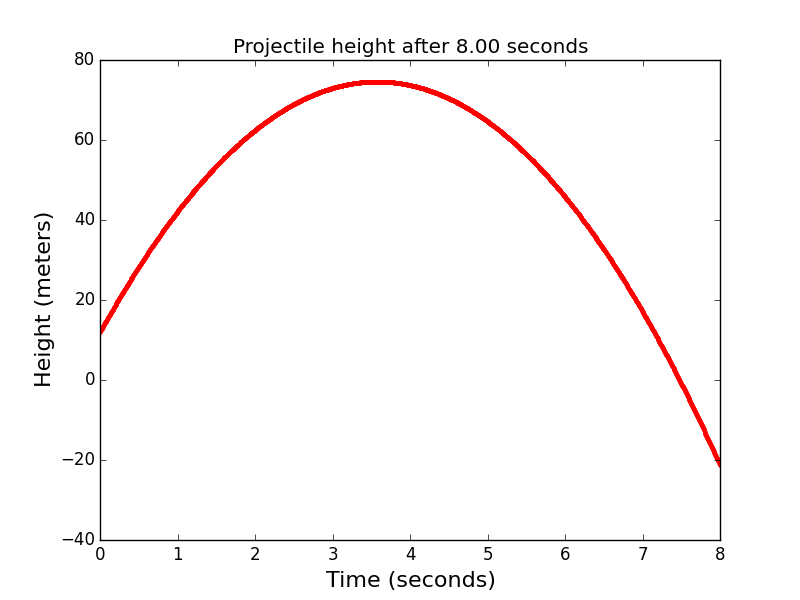
\includegraphics[scale=.5]{trial_1280.png}
\caption{A graph of the values for 1280 time steps}
\end{figure}
\section{Code}

\begin{verbatim}
#Colt Bradley
#2.4.16
#Homework 8

#import modules
import numpy as n
import pylab as p

#define variables from then homework
g = 9.8
y_0 = 12.
v_0 = 35.
t_0 = 0
t_f = 8.
nts = 1280
dt = (t_f - t_0)/nts

#create arrays
t = n.linspace(t_0, t_f,num = nts+1)
Y = n.zeros(len(t))
V = n.zeros(len(t))

#name the first elements of each array the initial value
Y[0] = y_0
V[0] = v_0

#creat the for loop that actually solves the equation. 
for i in range(0,nts):
    Y[i+1] = Y[i] + V[i]*dt
    V[i+1] = V[i] - g*dt

#Actual Value
t1 = v_0/g
y1 = -.5*g*t1**2 + v_0*t1 + y_0
t2 = 8-t1
y2 = (.5*g*t2**2)
actual = y1-y2
print actual #result of the above calculation
print Y[nts] #Result from iteration
error = (actual - Y[nts])/actual #calculated Error
print error

#build plot
p.plot(t,Y,"r")
p.plot(t,Y,"r.")
title = "Projectile height after {:.2f} seconds" .format(t_f)
p.xlabel("Time (seconds)", fontsize = 16)
p.ylabel("Height (meters)",fontsize = 16)
p.title(title)
p.show()
fig = "trial_{}" .format(nts) #Saves each plot with the number of time steps
p.savefig(fig+".png")
\end{verbatim}


\end{document}